% Chapter 3

\chapter{Preliminary analysis} % Main chapter title
\label{Chapter3}
As a precursor to the methodology discussion in the next chapter, we first present a preliminary analysis of the dataset.

\subsection{Daily play patterns}

Track plays, grouped into 30 min intervals, demonstrate a clear daily pattern with usage hitting the peak at around 5pm and a trough at around 6am.

\begin{figure}[h!]
	\centering
	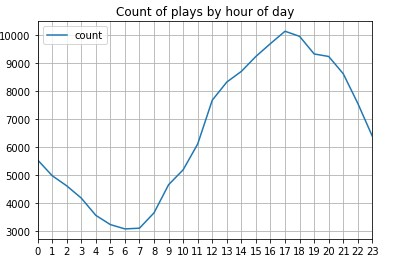
\includegraphics[width=7cm, keepaspectratio,]{fig004.jpg}
	\caption{5-5.30pm is peak listening time}
	\label{3a}
\end{figure} 

The peak of 5pm is likely explained by people finishing work at 5pm, however the bothdecline during pre-work hours of 6-8am was unexpected and may be a product of how the data was gathered.

Zooming out to view the pattern across an entire week in figure \ref{3b}, we see that the daily pattern occurs across every day of the week with weekends having a lower total number of plays.

\begin{figure}[h!]
	\centering
	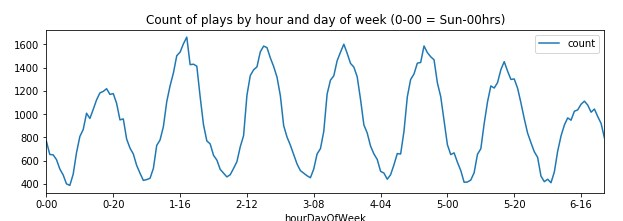
\includegraphics[width=7cm, keepaspectratio,]{fig005.jpg}
	\caption{Most popular times to listen to music across all users}
	\label{3b}
\end{figure} 

If we then select two random at users we can see how strong these patterns are over a period of week. Figure \ref{3c} shows that the daily patters are still discernable at the individual user level although they are not as clear cut. This demonstrates why models developed using aggregate level data may not translate well to individual user prediction. 

\begin{figure}[h!]
	\centering
	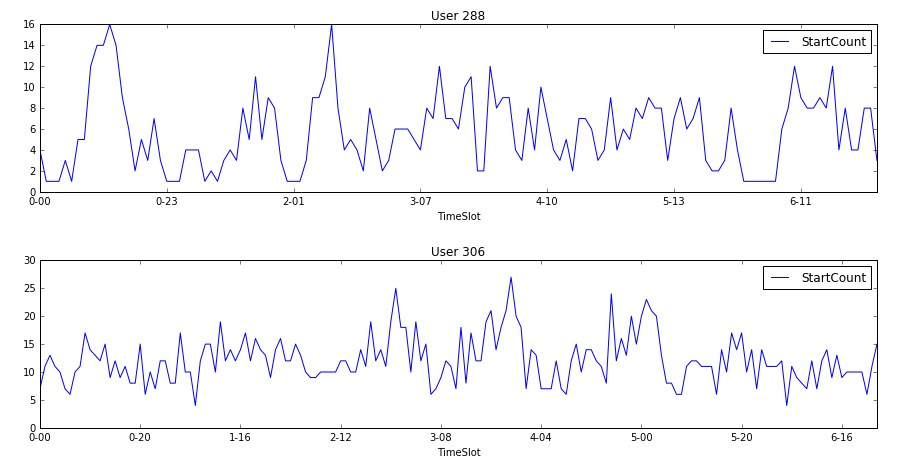
\includegraphics[width=7cm, keepaspectratio,]{fig006.jpg}
	\caption{Most popular times to listen to music by individual user}
	\label{3c}
\end{figure} 

\subsection{Unbalanced data}
The dataset is highly imbalanced with approximately 8.4% of periods being a play event. As we see later in the report, this has a breading on the results particularly on the RNN model.

\subsection{Inter-event times}

The dataset contains a timestamp associated with each user. This does not necessarily mean the user played a song in its entirety. Analysis shows plenty of cases where the interval time between tracs was a few seconds suggesting the user skipped tracks. 

Figure \ref{3d} shows a frequency plot of intervals. Intervals beyond 30 minutes continue the exponential decrease and are not shown. We see that while the mode is on par with a typical song length, there is a significant number of plays that lasted under 5 minutes. 

\begin{figure}[h!]
	\centering
	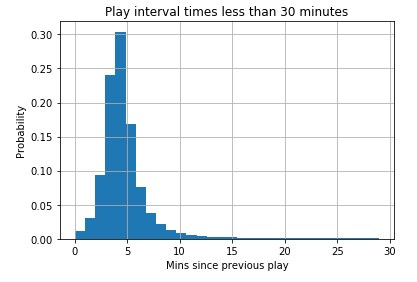
\includegraphics[width=7cm, keepaspectratio,]{fig003.jpg}
	\caption{}
	\label{3d}
\end{figure} 

For our purposes these are include as evidence that the user was interested in playing music at time $t$.

We can also assume that the song plays are not independent of one another, in that the probability of a play event at time t+1 is significantly higher if there was an event at time t. 


\subsection{Outliers}

The data was checked for any unusual outliers that may impinge upon the goal of developing a model to predict user behaviour. An analysis of plays by user reveals a high amount of variance between users on how many tracks are played. 

[***TODO: Replace with scatter plot***]

\begin{figure}[h!]
	\centering
	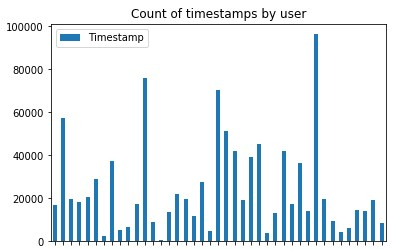
\includegraphics[width=7cm, keepaspectratio,]{fig002.jpg}
	\caption{Total play count by user}
	\label{fig:fig2}
\end{figure} 


\newpage

Further analysis showed one user in particular with very high amount of plays, with very low durations, suggesting it was likely to have been generated by a bot, possibly a LastFM test. This was excluded from the dataset.


\subsection{Summary}

The data follows a strong daily pattern at the aggregate level as well as the individual level, albeit to a lesser extent. Therefore the time of the day or most recent 24 hours is likely to be a strong predictor. Weekends have been sene to exhibit differences to weekdays so the day of the week is also a good feature. The data is high unbalanced and consists of a low amount of plays to non-plays, which are on averages around 5-6 minutes in duration.
